\section{Invariant Attacks -- Round Constants}
\begin{frame}
    \centering
    \Huge
    Invariant Attacks
    \vfill
\end{frame}

\begin{frame}{Invariant Attacks}
    \begin{block}{Main Idea: Invariant Subspaces}
        \centering
        \vspace{0.25em}
        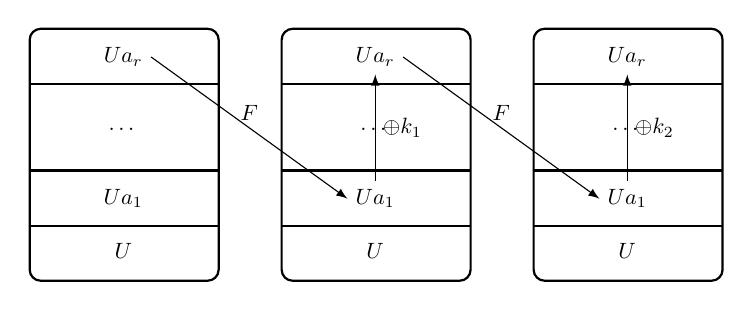
\begin{tikzpicture}[scale=0.8]
            \tikzstyle{every node}=[transform shape];

            \node (left-space) [draw,rectangle,thick,rounded corners,minimum width=3cm,minimum height=4cm,fill=white] at (1,0) {};
            \draw[thick] (left-space.west)+(0,1.125cm) -- node[above, yshift=1.5mm] (uar1) {$\coset{U}{a_r}$} +(3cm,1.125cm);
            \draw[thick] (left-space.west)+(0,-0.25cm) -- node[above, yshift=5mm] {\dots} +(3cm,-0.25cm);
            \draw[thick] (left-space.west)+(0,-1.125cm) -- node[above, yshift=1.5mm] {$\coset{U}{a_1}$}
                                                           node[below, yshift=-1.5mm] {$U$} +(3cm,-1.125cm);

            \node (middle-space) [draw,rectangle,thick,rounded corners,minimum width=3cm,minimum height=4cm,fill=white] at (5,0) {};
            \draw[thick] (middle-space.west)+(0,1.125cm) -- node[above, yshift=1.5mm] (uar2) {$\coset{U}{a_r}$} +(3cm,1.125cm);
            \draw[thick] (middle-space.west)+(0,-0.25cm) -- node[above, yshift=5mm] {\dots} +(3cm,-0.25cm);
            \draw[thick] (middle-space.west)+(0,-1.125cm) -- node[above, yshift=1.5mm] (ua12) {$\coset{U}{a_1}$}
                                                           node[below, yshift=-1.5mm] {$U$} +(3cm,-1.125cm);

            \draw[-latex] (uar1.east) -- node[above] {$F$} (ua12.west);
            \draw[-latex] (ua12.north) -- node[right] {$\oplus k_1$} (uar2.south);

            \visible<2->{%
            \node (right-space) [draw,rectangle,thick,rounded corners,minimum width=3cm,minimum height=4cm,fill=white] at (9,0) {};
            \draw[thick] (right-space.west)+(0,1.125cm) -- node[above, yshift=1.5mm] (uar3) {$\coset{U}{a_r}$} +(3cm,1.125cm);
            \draw[thick] (right-space.west)+(0,-0.25cm) -- node[above, yshift=5mm] {\dots} +(3cm,-0.25cm);
            \draw[thick] (right-space.west)+(0,-1.125cm) -- node[above, yshift=1.5mm] (ua13) {$\coset{U}{a_1}$}
                                                           node[below, yshift=-1.5mm] {$U$} +(3cm,-1.125cm);

            \draw[-latex] (uar2.east) -- node[above] {$F$} (ua13.west);
            \draw[-latex] (ua13.north) -- node[right] {$\oplus k_2$} (uar3.south);
            }
        \end{tikzpicture}
    \end{block}
    \visible<3->{%
    \begin{block}{Invariant Subspace Attacks~\cite{C:LAAZ11} (CRYPTO'11)}
        \vspace{0.25em}
        Let $U \subseteq \F_2^n$, $c, d \in U^\perp$, and $F : \F_2^n \to \F_2^n$.
        Then $U$ is an \emph{invariant subspace} (IS) if and only if
            $F(\coset{U}{c}) = \coset{U}{d}$
        and all round keys in $\coset{U}{(c+d)}$ are \emph{weak keys}.
    \end{block}
    }
\end{frame}

\begin{frame}{Invariant Attacks}{A Short History}
\begin{timeline}
\Task[\cite{C:LAAZ11}]{Publication of IS attack, breaking \printcipher/}
\Task[\cite{EC:LeaMinRon15}]{Generic Algorithm to find ISes, breaking \robin/, \iscream/, \zorro/}
\Task[\cite{ToSC:GJNQSM16}]{IS attack breaking \midori/64}
\Task[\cite{AC:TodLeaSas16}]{Invariant Set generalisation, breaking \scream/, \iscream/, \midori/64}
\Task[\cite{C:BCLR17}]{Proving resistance for Invariant attacks}
\end{timeline}
\end{frame}

\begin{frame}{Invariant Attacks}{Proving Resistance}
    \centering
    \begin{block}{\textbf{Goal}: Apply security argument from}
    \begin{quote}
        \fullcite{C:BCLR17}.
    \end{quote}
    \end{block}
    \begin{exampleblock}{What do we get from this?}
        \begin{itemize}
            \item Non-existence of invariants for both parts of the ronud function (S-box and linear layer)
        \end{itemize}
    \end{exampleblock}
    \begin{alertblock}{Issues}
    \begin{itemize}
        \item Other partitionings of the round function might allow invariants (Christof B\@. found examples)
        \item Not clear how to prove the general absence of invariant attacks (best we can currently prove)
        \item All known attacks exploit exactly this structure (splitting in S-box and linear layer)
    \end{itemize}
    \end{alertblock}
\end{frame}

\begin{frame}{Invariant Attacks}{Recap Security Argument (I)}
    \begin{columns}
        \begin{column}{0.35\textwidth}
        \begin{block}{Observation}
            \begin{itemize}
                \item Invariants for the linear layer $L$ and round key addition have to contain special linear structures.
                \item Denote by $c_1, \dots, c_t$ the round constant differences for rounds with the same round key.
                \item Then the linear structures of any invariant have to contain $W_L(c_1, \dots, c_t)$.
            \end{itemize}
        \end{block}
        \pause
    \end{column}
    \begin{column}{0.6\textwidth}
    \begin{block}{Linear Structures}
        Let $f : \F_2^n \to \F_2$.
        Then its \emph{linear structures} are
        \vspace*{-5pt}
        \begin{equation*}
            \mathrm{LS} \coloneqq \set{a \given f(x) + f(x+a) \text{ is constant}}\;.
        \end{equation*}
        \vspace*{-15pt}
    \end{block}
    \begin{block}{The smallest $L$-invariant subspace}
        $W_L(c_1, \dots, c_t)$ is the \emph{smallest $L$-invariant subspace} of~$\F_2^n$ containing all~$c_i$
        \vspace*{-5pt}
        \begin{equation*}
            \Leftrightarrow \forall x \in W_L(c_1, \dots, c_t): L(x) \in W_L(c_1, \dots, c_t)
        \end{equation*}
        \vspace*{-15pt}
    \end{block}
    \pause
    \begin{exampleblock}{The simple case}
        If $W_L(c_1, \dots, c_t) = \F_2^n$, only trivial invariants for $L$ and key addition are possible (constant 0 and 1 function).
    \end{exampleblock}
    \end{column}
    \end{columns}
\end{frame}

\begin{frame}{Invariant Attacks}{Recap Security Argument (II)}
    \begin{block}{Application to \clyde/}
    \begin{columns}
        \begin{column}{0.55\textwidth}
        \begin{itemize}
            \item Find the important round constant differences:\\
                  {\small (the differences where the same tweakey is added)}
        \end{itemize}
        \end{column}
        \pause
            \begin{column}{0.45\textwidth}
            \begin{itemize}
                \item[] Set of RC differences $D$ below\\
                        with $\abs{D} = 20$
            \end{itemize}
            \end{column}
    \end{columns}
    \end{block}
    \pause
    \begin{columns}
        \begin{column}{0.45\textwidth}
            \missingfigure{overview of clydes encryption over all 12 rounds}
        \end{column}
        \pause
        \begin{column}{0.45\textwidth}
            \vspace*{-10pt}
            \begin{align*}
                D &= D_{\mathrm{TK}_0} \cup D_{\mathrm{TK}_1} \cup D_{\mathrm{TK}_2} \cup D_0\\[5pt]
                D_{\mathrm{TK}_0} &= \set{0 + W(5), 0 + W(11), W(5) + W(11)} \\
                D_{\mathrm{TK}_1} &= \set{W(1) + W(7)} \\
                D_{\mathrm{TK}_2} &= \set{W(3) + W(9)} \\
                D_{0} &= \set{a + b \given a, b \in D^\prime, a \neq b} \\
                D^\prime &= \set{W(0), W(2), W(4), W(6), W(8), W(10)}
            \end{align*}
        \end{column}
    \end{columns}
\end{frame}

\begin{frame}{Invariant Attacks}{Application to \clyde/}
    \begin{itemize}
        \item Computing $W_L$ is efficiently doable (takes $\approx$ 10 seconds on my laptop).
        \item For the round constants chosen for \clyde/, $\dim W_L(D) = 128 = n$.
    \end{itemize}
    \begin{itemize}
        \item Thus, we can apply:
              \begin{block}{Proposition~2 \cite{C:BCLR17}}
                  Suppose that the dimension of $W_L(D)$ is $n$.
                  Then any invariant $g$ is constant (and thus trivial).
              \end{block}
    \end{itemize}
    \begin{itemize}
        \item We conclude that we cannot find any non-trivial $g$ for \clyde/ which is at the same time invariant for the S-box layer and for the linear layer.
    \end{itemize}
\end{frame}

\begin{frame}{Invariant Attacks}{Improvable?}
    \begin{block}{Bounding the dimension of $W_L$,~\cite[Theorem~1]{C:BCLR17}}
        Given a linear layer $L$.
        Denote by $Q_i$ its \emph{invariant factors}.
        Then
        \begin{equation*}
            \max_{c_1, \dots, c_t \in \F_2^n} \dim W_L(c_1, \dots, c_t) = \sum_{i=1}^t \deg Q_i\;.
        \end{equation*}
    \end{block}
    \pause
    \begin{block}{Application to \clyde/}
    \begin{columns}
        \begin{column}{0.6\textwidth}
        \begin{itemize}
            \item Compute invariant factors of linear layer:
            \item This gives a lower bound on the number of rounds:
        \end{itemize}
        \end{column}
        \pause
        \begin{column}{0.35\textwidth}
        \begin{itemize}
            \item[] $4 \times (x^{32}+1)$
            \item[] 3 steps/6 rounds
        \end{itemize}
        \end{column}
    \end{columns}
    \pause
    \begin{columns}
        \begin{column}{0.475\textwidth}
            \begin{itemize}
                \item 3 stps/6 rnds: $\dim W_L(c_1,\dots,c_4) = \hphantom{1}96$
                \item 4 stps/8 rnds: $\dim W_L(c_1,\dots,c_8) = 128$
            \end{itemize}
        \end{column}
        \begin{column}{0.475\textwidth}
            \begin{itemize}
                \item 5 stps/10 rnds: $\dim W_L(c_1,\dots,c_{13}) = 128$
                \item 6 stps/12 rnds: $\dim W_L(c_1,\dots,c_{20}) = 128$
            \end{itemize}
        \end{column}
    \end{columns}
    \end{block}
\end{frame}

\section{Subspace Trails}
\begin{frame}
    \centering
    \Huge
    Subspace Trails

    {\Large
        Probability~1~Truncated Differentials
    }

    \vfill
\end{frame}
\begin{frame}{Subspace Trails}
    \begin{block}{Main Idea: Subspace Trails}
        \centering
        \vspace{0.25em}
        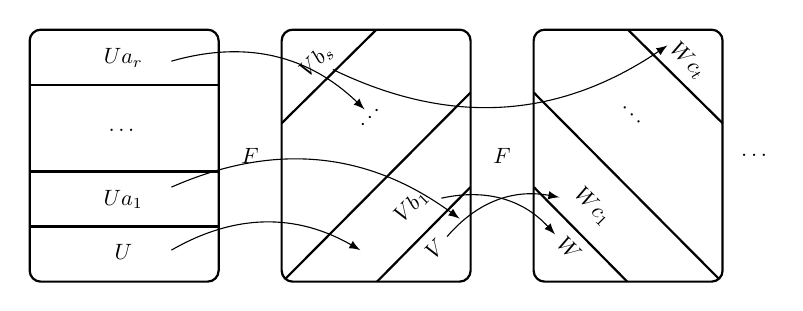
\begin{tikzpicture}[scale=0.8]
            \tikzstyle{every node}=[transform shape];

            \node (left2-space) [draw,rectangle,thick,rounded corners,minimum width=3cm,minimum height=4cm,fill=white] at (1,0) {};
            \draw[thick] (left2-space.west)+(0,1.125cm) -- node[above, yshift=1.5mm] {$\coset{U}{a_r}$} +(3cm,1.125cm);
            \draw[thick] (left2-space.west)+(0,-0.25cm) -- node[above, yshift=5mm] {\dots} +(3cm,-0.25cm);
            \draw[thick] (left2-space.west)+(0,-1.125cm) -- node[above, yshift=1.5mm] {$\coset{U}{a_1}$}
                                                            node[below, yshift=-1.5mm] {$U$} +(3cm,-1.125cm);

            \node (middle-space) [draw,rectangle,thick,rounded corners,minimum width=3cm,minimum height=4cm,fill=white] at (5,0) {};
            \draw[thick] (middle-space.north)+(0pt,-0.5pt) -- node[above, yshift=0.5mm, rotate=45] (vbs) {$\coset{V}{b_s}$} +(-1.5cm,-1.5cm);
            \draw[thick] (middle-space.east)+(-0.5pt,1cm) -- node[above, yshift=10mm, rotate=45] (middle-dots) {\dots} +(-3cm+1.25pt,-2cm+1.25pt);
            \draw[thick] (middle-space.east)+(-0.5pt,-5mm) -- node[above, yshift=2.5mm, rotate=45] (vb1) {$\coset{V}{b_1}$}
                                                        node[below, yshift=-0.5mm, rotate=45] (v) {$V$} +(-1.5cm,-2cm);

            \draw[-latex] (1.75,-1.5) to [bend left] (4.75,-1.5);
            \visible<2->{%
            \draw[-latex] (1.75,-0.5) to [bend left] (6.325,-1.0);
            \draw[-latex] (1.75,+1.5) to [bend left] (middle-dots);
            }

            \node (left-f) at (3,0) {$F$};

            \visible<3->{%
            \node (right-space) [draw,rectangle,thick,rounded corners,minimum width=3cm,minimum height=4cm,fill=white] at (9,0) {};
            \draw[thick] (right-space.north)+(0pt,-0.5pt) -- node[above, yshift=0.5mm, rotate=-45] (wct) {$\coset{W}{c_t}$} +(+1.5cm,-1.5cm);
            \draw[thick] (right-space.west)+(0.5pt,1cm) -- node[above, yshift=10mm, rotate=-45] (right-dots) {\dots} +(3cm-1.25pt,-2cm+1.25pt);
            \draw[thick] (right-space.west)+(0.5pt,-5mm) -- node[above, yshift=2.5mm, rotate=-45] (wc1) {$\coset{W}{c_1}$}
                                                        node[below, yshift=-0.5mm, rotate=-45] (w) {$W$} +(+1.5cm,-2cm);

            \node (middle-f) at (7,0) {$F$};
            \node (right-f) at (11,0) {$\ldots$};

            \draw[-latex] (vb1) to [bend left] (w);
            \draw[-latex] (v) to [bend left] (wc1);
            \draw[-latex] (vbs) to [bend right] (9.625,+1.75);
            }
        \end{tikzpicture}
    \end{block}
    \visible<3->{%
    \begin{block}{Subspace Trail Cryptanalysis~\cite{ToSC:GraRecRon16} (FSE'16)}
        \vspace{0.25em}
        \centering
        Let $U_0, \ldots, U_r \subseteq \F_2^n$, and $F : \F_2^n \to \F_2^n$.
        Then these form a \emph{subspace trail} (ST), $U_0 \through{F} \cdots \through{F} U_r$, iff
        \begin{equation*}
            \forall a \in U_i^\perp : \exists b \in U_{i+1}^\perp : \qquad F(\coset{U_i}{a}) \subseteq \coset{U_{i+1}}{b}
        \end{equation*}
    \end{block}
    }
\end{frame}

\begin{frame}{Computing Subspace Trails}
    \centering
    \begin{minipage}{0.45\textwidth}
    Given a starting subspace $U$, we can efficiently compute the corresponding longest subspace trail.

    \begin{lemma}
        \vspace{14pt}
        Let $U \through{F} V$ be a ST\@.
        Then for all $u \in U$ and all~$x$: $F(x) + F(x + u) \in V$.
        \vspace{14pt}
    \end{lemma}
    \end{minipage}
    \begin{minipage}{0.45\textwidth}
    \visible<2->{%
    \begin{block}{Proof}
        \centering
        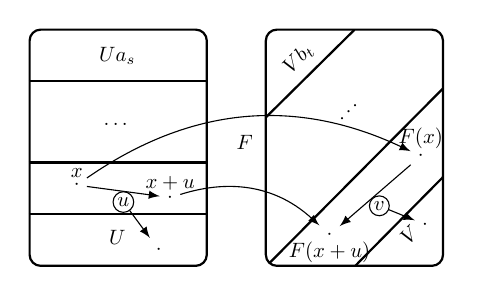
\begin{tikzpicture}[scale=0.75]
            \tikzstyle{every node}=[transform shape];

            \node (left2-space) [draw,rectangle,thick,rounded corners,minimum width=3cm,minimum height=4cm,fill=white] at (1,0) {};
            \draw[thick] (left2-space.west)+(0,1.125cm) -- node[above, yshift=1.5mm] {$\coset{U}{a_s}$} +(3cm,1.125cm);
            \draw[thick] (left2-space.west)+(0,-0.25cm) -- node[above, yshift=5mm] {\dots} +(3cm,-0.25cm);
            \draw[thick] (left2-space.west)+(0,-1.125cm) -- node[below, yshift=-1.5mm] {$U$} +(3cm,-1.125cm);

            \node (right2-space) [draw,rectangle,thick,rounded corners,minimum width=3cm,minimum height=4cm,fill=white] at (5,0) {};
            \draw[thick] (right2-space.north)+(0pt,-0.5pt) -- node[above, yshift=0.5mm, rotate=45] {$\coset{V}{b_t}$} +(-1.5cm,-1.5cm);
            \draw[thick] (right2-space.east)+(-0.5pt,1cm) -- node[above, yshift=10mm, rotate=45] {\dots} +(-3cm+1.25pt,-2cm+1.25pt);
            \draw[thick] (right2-space.east)+(-0.5pt,-5mm) -- node[below, yshift=-0.5mm, rotate=45] {$V$} +(-1.5cm,-2cm);

            \node[xshift=-20pt, yshift=-18pt] (x1) at (left2-space) {$\cdot$};
            \node[above] (x1-label) at (x1) {$x$};

            \node[xshift=32pt, yshift=-4pt] (y1) at (right2-space) {$\cdot$};
            \node[above] (y1-label) at (y1) {$F(x)$};

            \draw[-latex] (x1) to [bend left] node[below,yshift=-5pt] {$F$} (y1);

            \visible<3->{%
                \node[xshift=25pt, yshift=-24pt] (x2) at (left2-space) {$\cdot$};
                \node[above] (x2-label) at (x2) {$x+u$};

                \node[xshift=-12pt, yshift=-42pt] (y2) at (right2-space) {$\cdot$};
                \node[below] (y2-label) at (y2) {$F(x+u)$};

                \draw[-latex] (x1) -- node[below,draw,fill=white,inner sep=1pt,circle] (u-label) {$u$} (x2);
                \node[xshift=17pt, yshift=-23pt] at (u-label) (u) {$\cdot$};

                \draw[-latex] (u-label) -- (u);

                \draw[-latex] (x2) to [bend left] (y2);
            }

            \visible<4->{%
                \draw[-latex] (y1) -- node[below,xshift=2pt,draw,fill=white,inner sep=1pt,circle] (v-label) {$v$} (y2);
                \node[xshift=22pt, yshift=-9pt] at (v-label) (v) {$\cdot$};

                \draw[-latex] (v-label) -- (v);
            }

        \end{tikzpicture}
    \end{block}
    }
    \end{minipage}
    \visible<5->{%
    \begin{minipage}{0.925\textwidth}
    \begin{block}{Computing the subspace trail}
        \begin{itemize}
            \item To compute the next subspace, we have to compute the image of the derivatives.
        \end{itemize}
    \end{block}
    \end{minipage}
    }
\end{frame}

\begin{frame}{Computing Subspace Trails}{Algorithm}
    \centering
    \begin{minipage}{0.7\textwidth}
    \centering
    \begin{block}{Compute Subspace Trails}
    \begin{algorithmic}[1]
        \Require{A nonlinear, bijective function $F : \F_2^n \to \F_2^n$ and a subspace $U$.}
        \Ensure{The longest ST starting in $U$ over $F$.}
        \Statex{}
        \Function{Compute Trail}{$F$, $U$}
        \If{$\dim(U) = n$}
            \State{}\Return{$U$}
        \EndIf{}
        \State{}$V \leftarrow \emptyset$
        \For{$u_i$ basis vectors of $U$}
            \For{enough $x \in_\mathrm{R} \F_2^n$}\label{alg:compute_trail_1line}
                \Comment \eg/ $n+20$ $x$'s are enough
                \State{} $V \leftarrow V \cup \Delta_{u_i}(F)(x)$\label{alg:compute_trail_2line}
                \Comment $\Delta_a(F)(x) \coloneqq F(x) + F(x+a)$
            \EndFor{}
        \EndFor{}
        \State{}$V \leftarrow \mathrm{span}(V)$
        \State{}\Return{the subspace trail $U \rightarrow \textsc{Compute Trail}(F, V)$}
        \EndFunction{}
    \end{algorithmic}
    \end{block}
    \end{minipage}
\end{frame}

\begin{frame}{Subspace Trails}{Proving Resistance}
    \begin{block}{\textbf{Goal}: Apply security argument from}
    \begin{quote}
        \fullcite{ToSC:LeaTezWie18}.
    \end{quote}
    \end{block}
    \begin{exampleblock}{What do we get from this?}
        \begin{itemize}
            \item (Tight) upper bound on the length of any ST for an SPN construction
        \end{itemize}
    \end{exampleblock}
    \begin{alertblock}{Why is the \textsc{Compute Trail} algorithm not enough?}
        \begin{itemize}
            \item Exhaustively checking all possible starting points is to costly.
        \end{itemize}
    \end{alertblock}
\end{frame}

\begin{frame}{Subspace Trails}{How to bound the length of any subspace trail}
    \begin{columns}[t,onlytextwidth]
        \begin{column}{0.35\textwidth}
            \begin{block}{Observation\vphantom{g}}
                \vspace{0.5em}
                \centering
                \begin{tikzpicture}
                \foreach \z in {0,1,2,3} {%
                    \node[] (i\z) at ($(-0.25, \z*3em)+(0,0.35)$) {};
                    \node[] (o\z) at ($(0, \z*3em)+(3em,0.35)$) {};
                    \draw[thick,solid] (i\z) -- (o\z.center);
                }

                %% SBoxes
                \foreach \z in {0,1,2,3} {%
                    \node[draw,thick,solid,minimum width=2em,minimum height=2.75em,fill=white] (sl\z) at ($(i\z) + (2em,0em)$) {$S$};
                }

                \draw [draw=none] (i1) -- node[left,xshift=-0.5em] (U) {$U$} (i2);

                \draw [draw=none] (o1) -- node[right,xshift=0.5em] (V) {$V \ \ni$} (o2);
                \node [xshift=1em] at (V.east) {$\begin{pmatrix}0 \\ \\ \alpha \\ \\ 0 \\ \\ 0 \end{pmatrix}$} (o2);
                \end{tikzpicture}
                \vspace{0.5em}
            \end{block}
        \end{column}
        \begin{column}{0.6\textwidth}
            \visible<2->{%
            \begin{block}{Algorithm Idea}
                %\begin{minipage}[t][117.5pt][t]{\textwidth}
                \vspace{0.25em}
                Compute the subspace trails for any starting point $W_{i,\alpha} \in \mathcal{W}$, with
                    \begin{equation*}
                        W_{i,\alpha} \coloneqq (\underbrace{0, \ldots, 0}_{i-1}, \alpha, 0, \ldots, 0)
                    \end{equation*}
                %\end{minipage}
            \end{block}
            \begin{block}{Complexity (Size of $\mathcal{W}$)}
                \centering
                For an S-box layer $S : \F_2^{kn} \to \F_2^{kn}$ with $k$ S-boxes, each $n$-bit:\\
                $\abs{\mathcal{W}} = k \cdot (2^n-1)$
            \end{block}
            }
        \end{column}
    \end{columns}
\end{frame}

\begin{frame}{Subspace Trails}{Algorithm}
    \centering
    \begin{block}{Generic Subspace Trail Search}
    \begin{algorithmic}[1]
        \Require{A linear layer matrix $M : \F_2^{n \cdot k \times n \cdot k}$, and an S-box $S : \F_2^n \to \F_2^n$.}
        \Ensure{A bound on the length of all STs over $F = M \circ S^k$.}
        \Statex{}
        \Function{Generic Subspace Trail Length}{$M$, $S$}
        \State{}empty list $L$
        \For{possible initial subspaces represented by $W_{i,\alpha} \in \mathcal{W}$}
            \Comment Overall $k \cdot (2^n-1)$ iterations
            \State{}$L.\mathrm{append}(\textsc{Compute Trail}(S^k \circ M, \set{W_{i,\alpha}}))$
            \Comment $S^k$ denotes the S-box layer
        \EndFor{}
        \State{}\Return{$\max{\set{\mathrm{len}(t) \given t \in L}}$}
        \EndFunction{}
    \end{algorithmic}
    \end{block}

    \begin{block}{Overall Complexity}
        \centering
        \begin{tabular}{lccccc}
            \toprule
            Algorithm  & \textsc{Compute Trail} & \textsc{Generic Subspace Trail Length} &           Overall          &  \clyde/ & \shadow/ \\
            Complexity & $\mathcal{O}(k^2 n^2)$ &          $\mathcal{O}(k2^n)$           & $\mathcal{O}(k^3 n^2 2^n)$ & $2^{23}$ & $2^{29}$ \\
            \bottomrule
        \end{tabular}
    \end{block}
\end{frame}

%\subsection{Result}
%
%\begin{table}
%    \centering
%    \caption{%
%        Bound on the longest subspace trails in \clyde/ and \shadow/ (actual longest subspace trails can be one round longer).
%    }\label{tab:results_st}
%    \renewcommand{\arraystretch}{1.2}
%    \begin{tabular}{lcccc}
%        \toprule
%                 & \multicolumn{4}{c}{\cref{alg:generic}} \\
%        Cipher   & $r_e$   &   $d$   &    $r_d$   &  $d$  \\
%        \midrule
%        \clyde/  &   2     &    44   &      2     &   41  \\ \rowcolor{gray!10}
%        \shadow/ &  ???    &   ???   &     ---    &  ---  \\
%        \bottomrule
%    \end{tabular}
%\end{table}
%
%See \cref{tab:results_st}.

\section{Division Property}
\begin{frame}
    \centering
    \Huge
    Division Property
    \vfill
\end{frame}
\begin{frame}{Division Property}
    \begin{block}{\textbf{Goal}: Apply security argument from}
    \begin{quote}
        \fullcite{AC:XZBL16}.
    \end{quote}
    \end{block}
    \begin{exampleblock}{What do we get from this?}
        \centering
        bla
    \end{exampleblock}
    \begin{block}{Approach}
        \centering
        Model division trail propagations as MILP, find solutions for this over increasing number of rounds.
    \end{block}
\end{frame}

\section{Results}
\begin{frame}
    \centering
    \Huge
    Results
    \vfill
\end{frame}
\begin{frame}{Results}{Thanks for your attention!}
    \centering
    \begin{minipage}{0.5\textwidth}
    \begin{block}{Number of rounds}
    \centering
    \renewcommand{\arraystretch}{1.2}
    \begin{tabular}{ccc}
        \toprule
        Technique         & \clyde/ & \shadow/ \\
        \midrule
        Invariants        &   6     &   ---    \\ \rowcolor{saphierblau!20}
        Subspace Trails   & 2 (+1)  &  4 (+1)  \\
        Division Property &   8     &   ---    \\
        \bottomrule
    \end{tabular}
    \end{block}
    \begin{block}{Future Work/Cryptanalysis}
        \begin{itemize}
            \item Cryptagraph~\cite{ToSC:HalVej18}
            \item Post cryptanalysis results on mailinglist?
            \item Eprint Write-Up?
        \end{itemize}
    \end{block}
    \end{minipage}
    \begin{minipage}{0.45\textwidth}
        \centering
        \begin{figure}[!htb]
            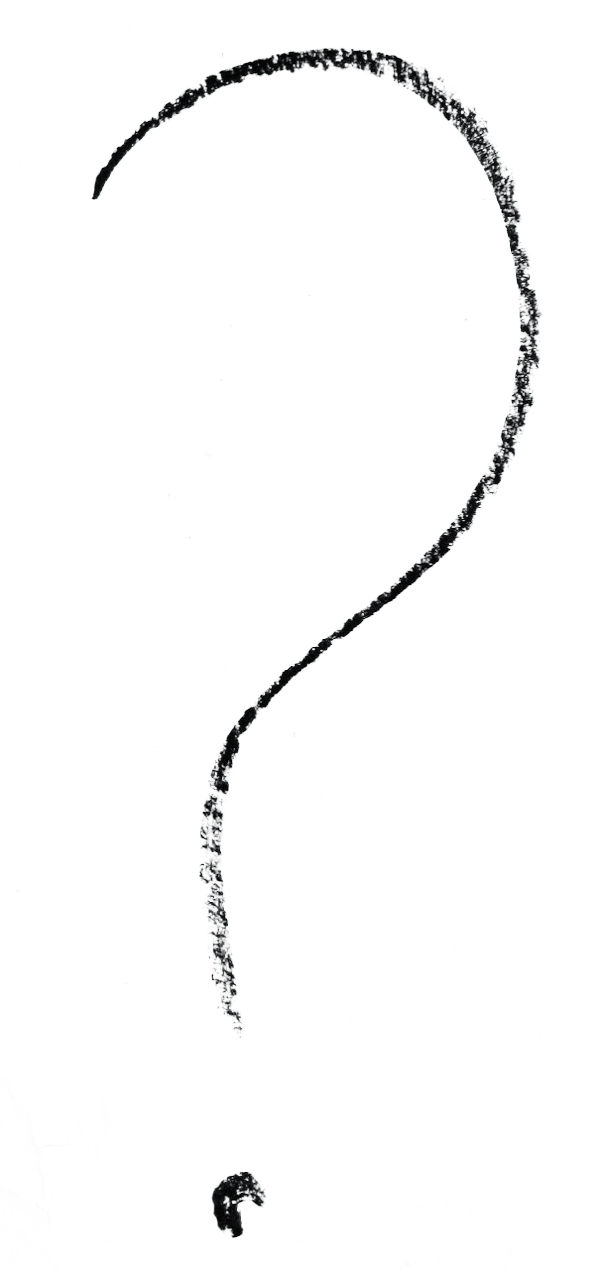
\includegraphics[height=50mm]{data/flickr/questionmark.png}
        \end{figure}
    \end{minipage}
\end{frame}

\begin{frame}[allowframebreaks]{References}
    \tiny
    \printbibliography{}
\end{frame}
